\documentclass[11pt, a4paper, oneside]{ctexart}
\usepackage{amsmath, amsthm, amssymb, appendix, bm, graphicx, hyperref, mathrsfs, float,subfigure,booktabs,tabularx,longtable,geometry,pdfpages}
%\usepackage{fancyhdr}	%用于更改默认的页眉页脚格式
\usepackage{listings}  % 用于插入代码
\usepackage{xcolor}  % 用于设置颜色
\usepackage{caption}

\captionsetup{font=small}
\renewcommand {\thetable} {\thesection{}.\arabic{table}}
\renewcommand {\thefigure} {\thesection{}.\arabic{figure}}

\title{\heiti\zihao{-1}\textbf{科学研究与创新实践开题报告}}
\date{}

\graphicspath{{img/}}
\bibliographystyle{plain}

\begin{document}

\begin{figure}
    \centering
    
\includegraphics[scale=1.2]{SJTU}
\end{figure}
\maketitle

\begin{table}[h]
    \centering
    \begin{tabular}{>{\bfseries\zihao{4}}c@{\zihao{4}\textbf{:}}>{\centering\arraybackslash\zihao{-4}}p{8cm}}
        题目 & 一种藤蔓式软体生长机器人的设计与控制 \\
        \cline{2-2}
        姓名 & 陈乐凯 \\
        \cline{2-2}
        学号 & 521020910180 \\
        \cline{2-2}
        导师 & 谷国迎 \\
        \cline{2-2}
        专业 & 机械工程 \\
        \cline{2-2}
        日期 & 2023.9.8 \\
        \cline{2-2}
    \end{tabular}
\end{table}
\thispagestyle{empty}

\newpage
\setcounter{page}{1}
\section{课题背景与研究目标}
在世界机器人领域蓬勃发展的今天,具有高灵活度和适应性的软体机器人是备受关注的领域之一,
其在环境勘测、生物医学、人机交互等领域的有着巨大的应用前景,其中,
一种类似藤蔓运动模式,依靠气动生长的机器人因其独特优势备受关注:
(1)通过气动反转材料,可以在不接触环境的情况下进行运动;
(2)气动的驱动模式在给予了该机器人足够刚度的同时又有一定的柔性,使得其能够适应各种复杂的工作环境,例如狭缝、流体等;
(3)由于机器人主体的薄膜材料本身的质量体积较小,使得其不仅便于收纳,又有很大的扩展延伸的潜力,在Hawkes等人的研究中\cite{hawkesSoftRobotThat2017a},这种生长机器人的最大长度能够达72米,最大生长速度达10米每秒,远远超过当前有类似功能的绳牵引机器人或尺蠖机器人;
(4)由于软体的特性,机器人对环境的破环较小\cite{coadRetractionSoftGrowing2020},具有在复杂环境勘测和生物医学检查领域应用的潜质;
(5)目前翻转式生长机器人的主体部分一般由聚丙烯塑料制成,成本和制造难度相对于一般刚性机器人低,结构较为简单,鲁棒性高。

\begin{figure}[h]
    \centering
    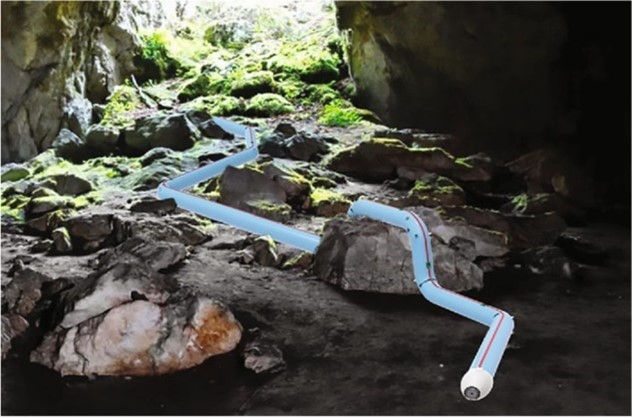
\includegraphics{fig1}
    \caption{类藤蔓的生长机器人概念设计}
    \label{fig-1}
\end{figure}

然而,这类生长机器人的连续性给其控制与建模带来了困难,
例如,由于反转生长的模式限制,难以加入复杂的驱动器(如气动肌肉,绳牵引)
对机器人进行主动运动控制,只能通过对表面材料进行直接处理预设运动轨迹,
并且由于生长机器人材料不断外翻,使得在顶端添加传感器较为困难,
目前研究者们聚焦于几个问题:
(1)如何在保持生长机器人结构和原理的情况下为机器人添加驱动器,实现自主运动控制;
(2)如何在外翻的顶部附加随动传感器(3)如何对已经产生变形的生长机器人进行回收,而不发生不可预测的屈曲。在转向问题上,Hawkes等人使用插销\cite{hawkesSoftRobotThat2017a},
通过在顶端释放预压缩的材料使两侧产生长度差,
从而实现转向(如图\ref{fig-2}A),这种方式响应时间长并且过程不可逆,
不适合推广应用,而Greer等人采用在机器人身体安装一系列气动人工肌肉(sPAMs)\cite{kublerMultiSegmentSoftGrowing2023},
通过充气收缩方式实现导航(如图\ref{fig-2}B),这种方式的机构数量多、体积小、精度要求高、加工难度大,
文章中只展现了二维简单路径的控制,
在此基础上Pengchun Li等人也提出利用四对电磁铁实现双模式八向运动控制,
提供了另一种可行方案(如图\ref{fig-2}C)。在传感器的添加上,
Hawkes最初的方案中采用单一绳牵引约束的方式在前端固定了一个用于导航的摄像头,
但是其稳定性和可靠程度较低,而Greer的论文中同时提出的一种滚轧式的顶端结构(如图\ref{fig-3}),
是目前一种可行性和和可靠度较高的方案。在生长机器人回收方面,
Margaret M. Coad等人证明了单一的绳牵引回收会导致不可预测的屈曲,
而不会保持稳定的翻转,并提出与Greer类似的滚轮结构进行顶端的主动回收(如图\ref{fig-4}),
因此有望在使用单一结构同时解决回收和传感器安装两大问题。

为了对生长机器人实现主动控制,一种准确合理的建模是不可或缺的。
由于模型的建立与机器人转向的方式有着紧密的联系,因此在完成结构设计后,
需要提出对应的数学模型,经过嵌入式系统处理,并推动驱动器工作,
最终实现探测传感-数据处理-驱动控制的任务。

\begin{figure}[h]
    \centering
    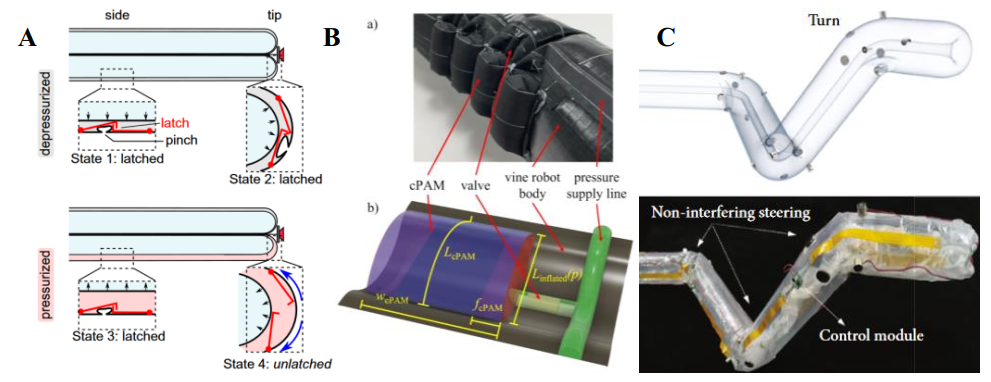
\includegraphics[scale=0.8]{fig2}
    \caption{各种转向方式的实现原理(A)插销式转向结构(B)附着在主体上的气动肌肉(sPAMs)及其结构(C)电磁铁转向结构}
    \label{fig-2}

    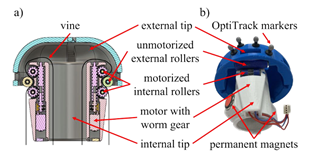
\includegraphics[scale=1.1]{fig3}
    \caption{带驱动滚轮的电动尖端支架}
    \label{fig-3}
\end{figure}

\begin{figure}
    \centering
    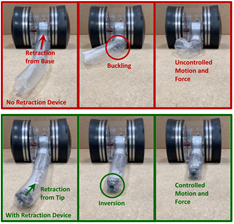
\includegraphics[scale=1.2]{fig4}
    \caption{气动机器人在回收过程中发生屈曲以及顶端主动回收机构}
    \label{fig-4}
\end{figure}
    
\section{主要研究内容与计划}
\subsection{基本原理的复现与改进}
翻转式生长机器人依靠内外压差和电机滚轴控制生长,
首先需要完成密封基座、电机滚筒、气泵安装的结构设计、并检查密封性,
实现基本的翻转生长,在此基础上通过对特定位置材料长度的设计,
实现预定轨迹的生长以及在多种环境交互下的被动适应性生长,
测量气压、生长速度、扭矩、机器人刚度等相关指标,寻找控制生长的最佳气压和扭矩。

首先,在生长过程中需要保持基座和生长机器人主体中的压强不变,
但由于整体容积变化、结构设计的缺陷、外部受到环境挤压等都可能导致内部气压变化,
希望设计一个系统对其进行压力的稳定控制。其次,在控制机器人生长于否的基础上,
还可以对其生长的长度进行控制,通过对滚筒旋转角度和圈数的设置,使其输出特定的长度。

\subsection{顶端传感器固定相关结构设计}
在实际勘探、医用的过程中,有对于前端安装如摄像头等传感器件的需求,
而对于这种前端并不固定的机器人来说,实现这个目标具有一定的挑战性,
因此希望参考前面学者已经提出的滚轧式的顶端结构,将传感器稳定地固定在前端,
后续还能够结合主动转向控制和计算机视觉实现自主导航。

\subsection{回收方案设计}
目前的实验和研究表明,通过直接施加绳牵引力使生长机器人回收的方式会导致主体的屈曲,
Margaret M. Coad等人提供了一种同样也是在顶端的主动回收机构,
考虑可以和顶端传感器固定的相关机构结合,实现传感-回收一体的方案设计。

\subsection{主动转向控制驱动器和控制方案的设计}
对于一体式的翻转生长机器人,由于其需要折叠回收,
无法通过复杂的刚性结构为转向提供驱动力,又因为其刚度较小,
不便于利用绳牵引等形式进行控制,且由于主体只存在单一的气腔,
而多个气腔并行的形式也只能提供单一的曲率,无法对于机器人各个部位进行单独的曲率控制,
目前可行的方案类似于Greer论文中提到的气动人工肌肉(sPAMs)的设计,
因此想要实现主动方向控制也是当前这类生长机器人面临的一大难题和挑战。

\subsection{转向控制建模}
实现转向控制之后,需要对转向关节处进行建模,
不论是插销、气动肌肉(sPAMs)还是电磁铁的设计,
其主要原理都是改变主体一侧的材料长度,通过对侧的长度差实现转向,
因此目前的建模方式就是将长度差作为转弯弧长差,再结合主体直径计算转弯角度,
知道了单一关节的转弯角度,最后就能够实现主动控制。

\section{预期收获}
《科学研究与创新实践》的课程提供了一次能够进入实验室体验科研过程的机会,
希望能在学长和老师的指导下较为独立的完成课题的研究,
培养包括论文阅读和复现、方案整合优化、加工与制造等能力,
为以后的研究工作打下基础,此外,也希望通过对于软体机器人的研究,
深化对于机器人领域的认知和实践,掌握相关机器人原理、控制方式、建模方法,
也希望以后能进入机器人相关产品设计、系统及硬件开发行业工作。

\newpage
\bibliography{robot}

\end{document}